\section{Exercise 2}

\subsection{Instruction}

In this problem, we’ll examine the effects of clock frequency bias on Doppler
derived from frequency downconversion and sampling.

Usually, we don’t measure signal properties directly at the signal’s incoming
frequency. Instead, we convert incoming signals to a lower center frequency by a
process called frequency conversion. To understand frequency conversion, recall
that

\begin{equation}
	cos(x) cos(y) = \frac{1}{2} [cos(x − y) + cos(x + y)]
\end{equation}

Hence, by multiplying an incoming signal $x(t) = cos(2 \pi f_c t)$ by a local
signal $x_l(t) = 2 cos(2 \pi f_l t)$ and then low-pass filtering the result to
eliminate the high frequency $f_c + f_l$ component, we convert the high frequency
signal down to a lower frequency $f_b = f_c − f_l$. Processes such as
amplification, transmission, filtering, delaying, recording, and sampling are
easier to do at lower frequencies. Figure~\ref{fig:ex2_diagram} shows a diagram
of the frequency conversion process.

\begin{figure}[H]
	\centering
	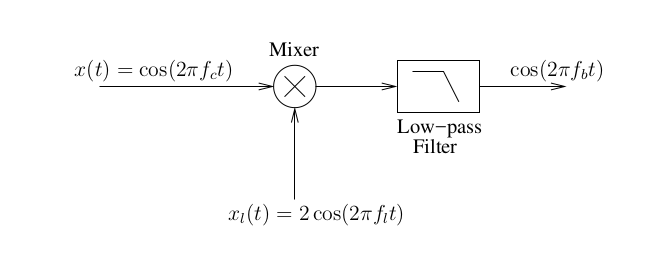
\includegraphics[width=0.9\textwidth]{figs/ex2_diagram.png}
	\caption{A single-stage frequency conversion (mixing) operation.}
	\label{fig:ex2_diagram}
\end{figure}

Assume that some oscillator with a perfect clock produces a pure sinusoid of the
form $x(t) = cos(2 \pi f_c t)$. Suppose that you receive this signal and make a
measurement $f_m$ of the signal’s frequency by (1) performing frequency
conversion to translate the signal to a nominal center frequency $f_{b,nom} = 0 Hz$
and then (2) sampling the signal with nominal sampling interval $\Delta t$ and
observing the number of samples per period. Assume there is no motion between
your receiver and the signal transmitter. Suppose that the local clock you’re
using to perform frequency conversion and sampling has a fractional frequency
error of $\Delta f /f < 0$.

Derive an expression for the apparent Doppler $f_D$ resulting from frequency
conversion and sampling with a clock that has this fractional frequency error.
Express your result in terms of $f_c$ and $\Delta f /f$. How does this expression
differ from the one derived in problem 3?

Note that if $f_l < f_c$, as will be the case for our problem because
$\Delta f /f < 0$, then $f_b > 0$. This is an example of low-side mixing. But if
$f_l > f_c$, then $f_b < 0$; this is high-side mixing. What would be the meaning
of a signal for which $f_b < 0$? Upon sampling a signal with $f_b < 0$ to
determine the period, would we measure a negative frequency?


\subsection{Result}

\begin{equation}
	x(t) * x_l(t) = 2 cos (2 \pi f_c t) cos(2 \pi f_l t))
\end{equation}

\begin{equation}
	x(t) * x_l(t) =  cos (2 \pi (f_c - f_l) t) + cos(2 \pi (f_c + f_l) t)
\end{equation}

After applying the low-pass filter we get

\begin{equation}
	x_{LPF}(t) = cos (2 \pi (f_c - f_l) t)
\end{equation}

Let's clarify:

\begin{equation}
	f_b = f_c - f_l = f_c - (f_{l,nom} + \Delta f)
\end{equation}

We know that $f_{b,nom} = 0 Hz$. Therefore, $f_{l,nom} = f_c$.

Now, it's necessary to focus on the last part of the processing (sampling). For
that, lets write the following relationships.

\begin{equation}
	\frac{\Delta f}{f_{l,nom}} = \frac{f_l - f_{l,nom}}{f_{l,nom}}
	= \frac{f_l}{f_{l,nom}} - 1
	= \frac{\Delta t_{l,nom}}{\Delta t_l} - 1
\end{equation}


\begin{equation}
	\Delta t_{l,nom} = (\frac{\Delta f}{f_{l,nom}} + 1) \Delta t_l
\end{equation}

Since the objective at this stage is to measure the frequency of the signal that
comes from the low-pass filter, it is safe to say that we are trying to measure
$f_b$. Thus, $f_b = \frac{1}{N*\Delta t_l}$.

\begin{equation}
	f_m = \frac{1}{N * \Delta t_{l,nom}}
	= \frac{1}{N *(\frac{\Delta f}{f_{l,nom}} + 1) \Delta t_l}
	= \frac{f_b}{\frac{\Delta f}{f_{l,nom}} + 1}
\end{equation}

Since it was stablished that $f_{l,nom} = f_c$.
Then, $\Delta f = f_c \frac{\Delta f}{f_{l,nom}}$

\begin{equation}
	f_m = \frac{\frac{\Delta f}{f_{l,nom}} f_c}{\frac{\Delta f}{f_{l,nom}} + 1}
\end{equation}

Finally, it is possible to reason that the measured frequency is the very
apparent Doppler $f_D$ (with a changed sign). This is because the frequency
conversion already applied the following substraction $f_b = f_c - f_l$, which
is almost the same substraction needed for $f_D = f_l - f_c$.

\begin{equation}
	f_D = -\frac{\frac{\Delta f}{f_{l,nom}} f_c}{\frac{\Delta f}{f_{l,nom}} + 1}
\end{equation}

Q: How does the expression differ from the one derived in problem 3?
A: It doesn't. It's the same relationship.

Q: What would be the meaning of a signal for which $f_b < 0$?
A: It would mean that the apparent Doppler would be inverted. Therefore, we
would think that the TX and RX are getting further and further appart.

Q: Upon sampling a signal with $f_b < 0$, would we measure a negative frequency?
A: No, we would measure the absolute value of $f_b$.

